\documentclass[tikz,border=10pt]{standalone}
\usepackage{amsmath,amssymb}
\usepackage{newpxtext,newpxmath}
\usetikzlibrary{arrows.meta,decorations.pathreplacing,calc}

\definecolor{inkDark}{HTML}{1E293B}
\definecolor{slateSub}{HTML}{334155}
\definecolor{pathBlue}{HTML}{005A9C}
\definecolor{accentRed}{HTML}{B91C1C}
\definecolor{accentTeal}{HTML}{0E6251}
\definecolor{accentAmber}{HTML}{B45309}
\definecolor{bandBlue}{HTML}{DBEAFE}
\definecolor{boxFill}{HTML}{F8FAFC}

\begin{document}
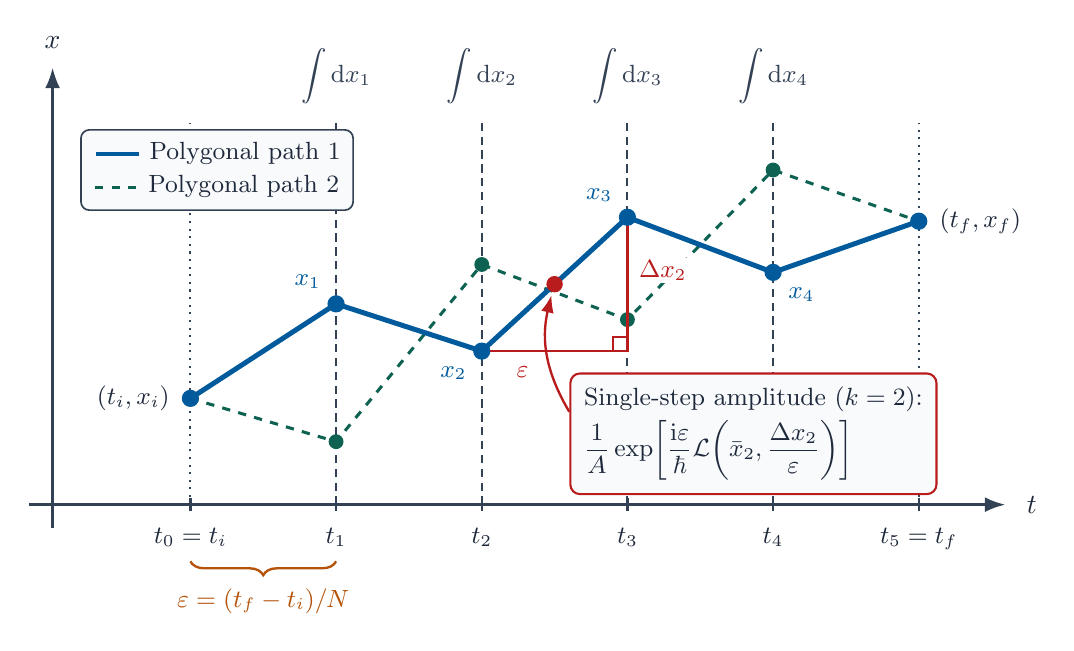
\begin{tikzpicture}[
    >=Latex,
    every node/.style={font=\normalsize, text=inkDark},
    axis/.style={-{Latex[length=2.6mm,width=1.9mm]}, line width=0.95pt, draw=slateSub},
    sliceline/.style={densely dashed, line width=0.7pt, draw=slateSub},
    ptBlue/.style={circle, fill=pathBlue, inner sep=2.2pt},
    ptTeal/.style={circle, fill=accentTeal, inner sep=1.9pt}
]

    % Axes
    \draw[axis] (-0.3, 0) -- (12.1, 0) node[right=4pt] {$t$};
    \draw[axis] (0, -0.3) -- (0, 5.55) node[above=3pt] {$x$};

    % Time slice x-coordinates: shifted right so (t_i, x_i) never crosses x-axis
    \def\tz{1.75}
    \def\ta{3.60}
    \def\tb{5.45}
    \def\tc{7.30}
    \def\td{9.15}
    \def\te{11.00}

    % Vertical integration slices
    \draw[dotted, line width=0.75pt, draw=slateSub] (\tz, 0) -- (\tz, 4.85);
    \draw[sliceline] (\ta, 0) -- (\ta, 4.85) node[above=3pt, font=\small, text=slateSub] {$\displaystyle\int\mathrm{d}x_1$};
    \draw[sliceline] (\tb, 0) -- (\tb, 4.85) node[above=3pt, font=\small, text=slateSub] {$\displaystyle\int\mathrm{d}x_2$};
    \draw[sliceline] (\tc, 0) -- (\tc, 4.85) node[above=3pt, font=\small, text=slateSub] {$\displaystyle\int\mathrm{d}x_3$};
    \draw[sliceline] (\td, 0) -- (\td, 4.85) node[above=3pt, font=\small, text=slateSub] {$\displaystyle\int\mathrm{d}x_4$};
    \draw[dotted, line width=0.75pt, draw=slateSub] (\te, 0) -- (\te, 4.85);

    % Time axis ticks & labels
    \foreach \xpos/\lbl in {\tz/{$t_0 = t_i$}, \ta/{$t_1$}, \tb/{$t_2$}, \tc/{$t_3$}, \td/{$t_4$}, \te/{$t_5 = t_f$}}{
        \draw[line width=0.8pt, draw=slateSub] (\xpos, 0.08) -- (\xpos, -0.08);
        \node[below=4pt, font=\small] at (\xpos, -0.04) {\lbl};
    }

    % Brace for step size \varepsilon
    \draw[decorate, decoration={brace, amplitude=5pt, mirror}, line width=0.85pt, draw=accentAmber]
        (\tz, -0.72) -- (\ta, -0.72)
        node[midway, below=6pt, font=\small, text=accentAmber] {$\varepsilon = (t_f - t_i)/N$};

    % Secondary polygonal path (teal, dashed) - routed cleanly above bottom-right box
    \coordinate (Q0) at (\tz, 1.35);
    \coordinate (Q1) at (\ta, 0.80);
    \coordinate (Q2) at (\tb, 3.05);
    \coordinate (Q3) at (\tc, 2.35);
    \coordinate (Q4) at (\td, 4.25);
    \coordinate (Q5) at (\te, 3.60);

    \draw[line width=1.1pt, draw=accentTeal, dashed]
        (Q0) -- (Q1) -- (Q2) -- (Q3) -- (Q4) -- (Q5);
    \foreach \p in {Q1,Q2,Q3,Q4}{
        \node[ptTeal] at (\p) {};
    }

    % Primary polygonal path (blue, solid) - raised slightly at P2, P3 for clean geometry
    \coordinate (P0) at (\tz, 1.35);
    \coordinate (P1) at (\ta, 2.55);
    \coordinate (P2) at (\tb, 1.95);
    \coordinate (P3) at (\tc, 3.65);
    \coordinate (P4) at (\td, 2.95);
    \coordinate (P5) at (\te, 3.60);

    \draw[line width=1.8pt, draw=pathBlue]
        (P0) -- (P1) -- (P2) -- (P3) -- (P4) -- (P5);

    % Right triangle highlighting segment k=2: (P2) -> (P3)
    \coordinate (Rcorner) at (\tc, 1.95);
    \draw[line width=1.0pt, draw=accentRed] (P2) -- (Rcorner) -- (P3);
    \draw[line width=0.75pt, draw=accentRed] ($(Rcorner)+(-0.18,0)$) |- ($(Rcorner)+(0,0.18)$);
    \node[below=2pt, font=\small, text=accentRed] at ($(P2)!0.28!(Rcorner)$) {$\varepsilon$};
    \node[right=3pt, font=\small, text=accentRed, fill=white, inner sep=1pt] at ($(Rcorner)!0.60!(P3)$) {$\Delta x_2$};

    % Midpoint dot on segment P2 -> P3
    \coordinate (Mid2) at ($(P2)!0.5!(P3)$);
    \node[circle, fill=accentRed, inner sep=2.1pt] at (Mid2) {};

    % Vertices of primary path
    \foreach \p in {P0,P1,P2,P3,P4,P5}{
        \node[ptBlue] at (\p) {};
    }

    % Endpoint labels (completely clear of axes!)
    \node[left=4pt, font=\small] at (P0) {$(t_i, x_i)$};
    \node[right=4pt, font=\small] at (P5) {$(t_f, x_f)$};

    % Vertex labels on primary path
    \node[above left=2pt, font=\small, text=pathBlue] at (P1) {$x_1$};
    \node[below left=2pt, font=\small, text=pathBlue] at (P2) {$x_2$};
    \node[above left=2pt, font=\small, text=pathBlue] at (P3) {$x_3$};
    \node[below right=2pt, font=\small, text=pathBlue] at (P4) {$x_4$};

    % Callout box cleanly placed in open lower-right whitespace
    \node[
        draw=accentRed, line width=0.75pt, rounded corners=3.5pt,
        fill=boxFill, inner sep=5pt, font=\small, text=inkDark, align=left
    ] (segbox) at (8.90, 0.90)
    {Single-step amplitude ($k=2$):\\[2pt]
     $\dfrac{1}{A}\exp\!\left[\dfrac{\mathrm{i}\varepsilon}{\hbar}\mathcal{L}\!\left(\bar x_2,\dfrac{\Delta x_2}{\varepsilon}\right)\right]$};

    \draw[-{Latex[length=2.2mm]}, draw=accentRed, line width=0.85pt]
        ($(segbox.west)+(0,0.28)$) to[bend left=22] ($(Mid2)+(-0.04,-0.14)$);

    % Legend in upper-left whitespace
    \node[
        draw=slateSub, line width=0.6pt, rounded corners=3pt,
        fill=boxFill, inner sep=4.5pt, font=\small, anchor=west, align=left
    ] at (0.35, 4.25) {
        \tikz[baseline=-0.5ex]{\draw[line width=1.6pt, pathBlue] (0,0)--(0.55,0);} Polygonal path 1\\[1pt]
        \tikz[baseline=-0.5ex]{\draw[line width=1.1pt, accentTeal, dashed] (0,0)--(0.55,0);} Polygonal path 2
    };

\end{tikzpicture}
\end{document}
